\section{Virtual Reality Data}
\label{S:T3}
For the purpose of this study, Virtual Immersive Reality Environment (VIRE) is used to simulate different scenarios and conduct experiments on different pedestrians safety and walking behaviour. Introduced in Farooq~\textit{et al.}~\citep{farooqvire}, VIRE uses Head Mounted Display and virtual reality to enable interactive, immersive and complex simulated scenarios. Hypothetical traffic simulations can be projected directly to eyes of users. In this study, we specifically focus on pedestrian crossing behaviour at unsignalized intersections, as a plausible scenario in the autonomous future. Participants are asked to cross the street in different scenarios.
Detailed experiments were conducted over a 3 month period in summer 2018, in four different places to cover a heterogeneous population. A total of 160 individuals from different age groups participated in the experiment. The experiments were performed at Ryerson University, City of Markham Public Library, Toronto City Hall, and North York Civic center. Participants were exposed to multiple scenarios, with changing parameters in each round. In Figure \ref{fig:exp}, an experiment and its components are shown.
\begin{figure}[!h]
\centering
\sbox{\measurebox}{%
  \begin{minipage}[b]{.4\textwidth}
  \subfloat
  {\label{fig:figA}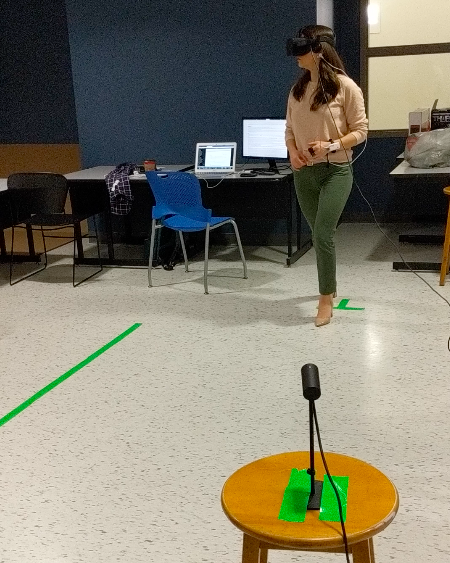
\includegraphics[width=0.91\textwidth,height=8cm]{chapter_6/figures/img1.png}}
    (a)
  \end{minipage}}
\usebox{\measurebox}\qquad
    \begin{minipage}[b][\ht\measurebox][s]{.4\textwidth}
    \centering
    \subfloat
    {\label{fig:figB}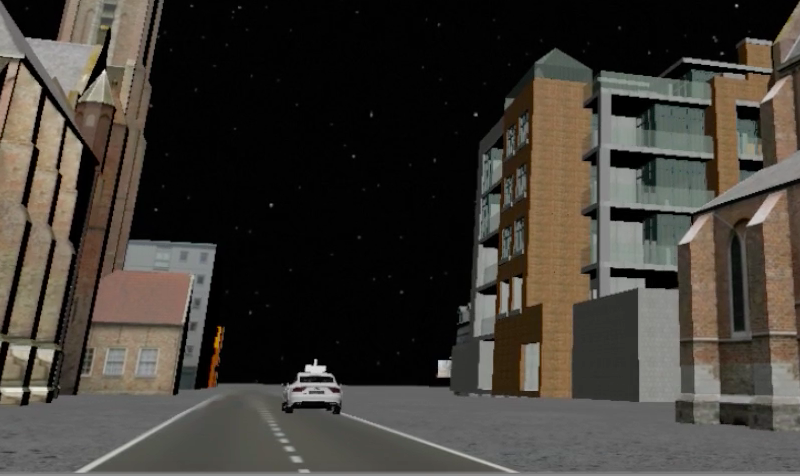
\includegraphics[width=0.91\textwidth,height=3.5cm]{chapter_6/figures/img3.png}}
    (b)
    \vfill
    \subfloat
    {\label{fig:figC}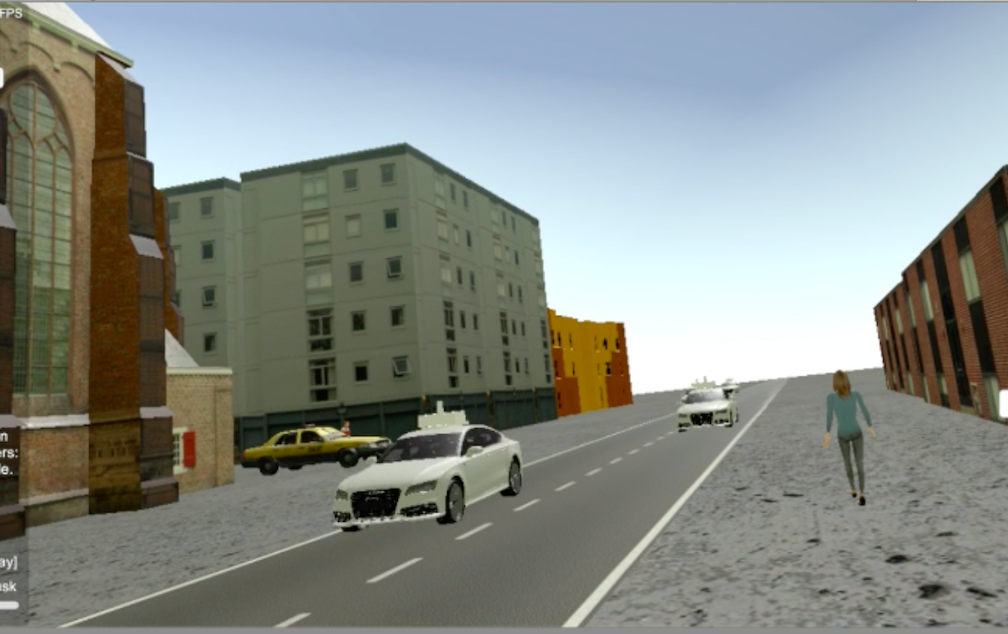
\includegraphics[width=0.91\textwidth,height=3.5cm]{chapter_6/figures/pic1.png}}
    (c)
    \end{minipage}
\caption{VR experiment. (a) A participant doing the experiment (b) A sample night view of the environment (c) A sample day view of the environment}
\label{fig:exp}
\end{figure}
While doing the experiment, pedestrians coordinates and head orientations, as well as simulated vehicles' positions are recorded every 100 milliseconds. Environmental context variables used as auxiliary input to the core LSTM network include type of road (one-way, two-way or two-way with median), speed limit (30, 40 or 50 km/hr), lane width (2.5, 2.75 or 3 m), weather conditions (snow day or clean), time of the day (day or night), and arrival rate of cars (530, 750, 1100 veh/hr). These variables are defined in a way that a self-driving car can capture and use them as input to its trajectory prediction algorithm. More information on other features used for the purpose of scenario generation and design of experiments can be found in ~\citep{kalatian2019deepsurvival}.  